% Display-only generated file; exact saved-number bindings are in notes/v12/new-paper-number-bindings.json.
\subsection{Why does regression lose at low frequency?}\label{sec:v12-low-frequency}
Figure~\ref{fig:v12-decomposition} splits full regression's actual excess into the selected report's gap from the best finite candidate and that candidate's gap from historical headroom. The best candidate uses evaluation hindsight over five finite penalties; the ordinary empirical option is excluded. For full regression, the finite-menu gap is positive in 29 of 41 short-history weekly cells; selection exceeds half of positive actual excess in 27. Both criteria hold, so benchmark advantages and selection losses coexist within this menu. Separate component medians need not add: actual excess is 19.44\%, selection 18.32\%, and the diagnostic gap 4.37\%.

This retrospective finite oracle is diagnostic, cannot guide deployment, and cannot rule out information in other conditional models. When validation selects the ordinary empirical limit, it can beat every finite candidate and make the selection component negative. Both long-history FX horizons have a negative finite-menu gap. Expanded menus also bring the calibrated simulation medians close to their historical reference, leaving the empirical frequency mechanism unidentified.

\begin{figure}[htbp]\centering
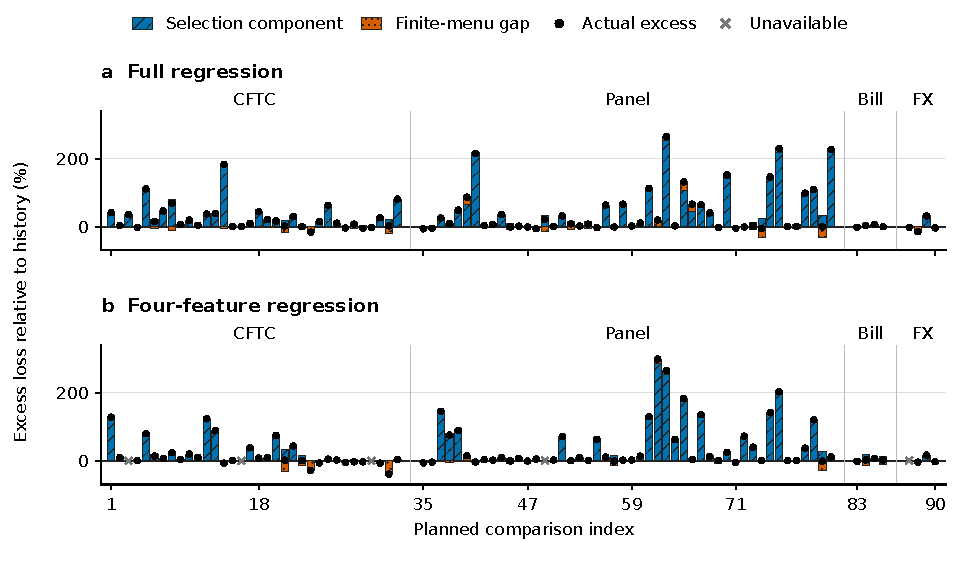
\includegraphics[width=.98\linewidth,height=2.75in,keepaspectratio]{figures/v12-decomposition.pdf}
\caption{Signed decomposition of regression excess loss against matched historical headroom, with selection in blue, the finite-menu diagnostic gap in orange, and actual excess as black dots. Crosses retain unavailable comparisons; the text focuses on short-history weekly cells while all planned comparisons remain plotted.}\label{fig:v12-decomposition}
\end{figure}

Extending validation from 52 to 156 weeks keeps the CFTC evaluation period, training histories, and refitting clock fixed. Median excess falls from 19.33\% to 4.03\% with 52-week training histories, and from 10.35\% to 0.53\% with 260-week histories. Infinite-penalty selections rise from 4 to 10 of 17 contracts, and from 4 to 5 of 17, respectively. These differences between across-contract medians need not match typical paired improvements and do not identify a causal effect. Four-feature failures remain unavailable in the complete inventory (Supplement Section S36).

Tail-level sensitivity remains incomplete, as Table~\ref{tab:v12-tau} shows for 90\% and 99\% quantiles under matched histories. At 99\%, historical headroom wins 28 of 34 CFTC comparisons; one failure leaves the 29-win threshold unresolved. Both FX periods remain unavailable at 99\%, leaving the combined improvement criterion undetermined. Unavailable planned comparisons are retained, and successful subsets never replace a missing full-group median.

\begin{table}[htbp]\centering\small
\caption{Full-regression relative excess loss (\%) at alternative quantile levels. Positive values favor matched historical headroom; NA retains any failed required comparison.}\label{tab:v12-tau}
\begin{tabular}{lrr}\toprule
Source / training history & 90\% & 99\% \\\midrule
CFTC, 52 weeks & +3.45 & +15.05 \\
CFTC, 260 weeks & +1.58 & \textsc{NA} \\
FX, original period & -10.15 & \textsc{NA} \\
FX, earlier period & -17.85 & \textsc{NA} \\
Treasury bills & +0.67 & +44.22 \\
\bottomrule\end{tabular}
\par\vspace{2pt}\begin{minipage}{.95\linewidth}\footnotesize
Contract rows report full-group medians. FX uses 2,880-hour training histories; Treasury uses 260 weeks. Successful subsets never replace a required full group.
\end{minipage}\end{table}
